\documentclass{beamer}


% For more themes, color themes and font themes, see:
% http://deic.uab.es/~iblanes/beamer_gallery/index_by_theme.html


\mode<presentation>
{
	\usetheme{Madrid}       % or try default, Darmstadt, Warsaw, ...
	\usecolortheme{wolverine} % or try albatross, beaver, crane, ...
	\usefonttheme{default}    % or try default, structurebold, ...
	\setbeamertemplate{navigation symbols}{}
	\setbeamertemplate{caption}[numbered]
} 

\usepackage{lmodern}
\usepackage[english]{babel}
\usepackage[utf8]{inputenc}
\usepackage{chemfig}
\usepackage[version=3]{mhchem}
\usepackage{amsmath}
\usepackage{mathtools}
\usepackage[absolute,overlay]{textpos}
\usepackage{graphicx}
\graphicspath{ {img/} }
\usepackage[absolute,overlay]{textpos}
\usepackage{bm}
\usepackage[normalem]{ulem}
\usepackage{cancel}
\usepackage{relsize}
\usepackage[export]{adjustbox}
\usepackage[T1]{fontenc}

\definecolor{ForestGreen}{rgb}{0.13, 0.55, 0.13}

\newcommand\norm[1]{\left\lVert#1\right\rVert}
\newcommand\red[1]{\textcolor{red}{\textbf{#1}}}
\newcommand\blue[1]{\textcolor{blue}{\textbf{#1}}}
\newcommand\yellow[1]{\textcolor{yellow}{\textbf{#1}}}
\newcommand\green[1]{\textcolor{ForestGreen}{\textbf{#1}}}
\DeclarePairedDelimiterX{\ip}[2]{\langle}{\rangle}{#1, #2}
\DeclareMathOperator*{\argmax}{\arg\!\max}

% On Overleaf, these lines give you sharper preview images.
% You might want to `comment them out before you export, though.
\usepackage{pgfpages}
\pgfpagesuselayout{resize to}[physical paper width=8in, physical paper height=6in]

% Here's where the presentation starts, with the info for the title slide
\title[Joint Training of CNN and PGM for HPE]{\textbf{Joint Training of a Convolutional Network and a Graphical Model for Human Pose Estimation}}
\subtitle{}
\author{Y.Fan \& M.Andriushchenko}
\institute{Saarland Univ.}
\date{30 January 2018}

\begin{document}
	
	% Title page
	\begin{frame}
		\titlepage
	\end{frame}


	\begin{frame}[c]
		\frametitle{What are we doing?}
		\begin{center}
			\blue{Task}: \textbf{single person pose estimation} from 2D images \\
		\end{center}
	\end{frame}
	
	\begin{frame}[c]
		\frametitle{What are we doing?}
		\begin{center}
			\blue{Task}: \textbf{single person pose estimation} from 2D images \\
			\blue{Method:} combination of a CNN and a PGM trained end-to-end jointly \\ \ \\
		\end{center}
	\end{frame}


    \begin{frame}[c]
        \frametitle{Modern computer vision}
        \begin{center}
        	\blue{CNNs} is the method of choice for many computer vision tasks. \\            
            \begin{figure}
            	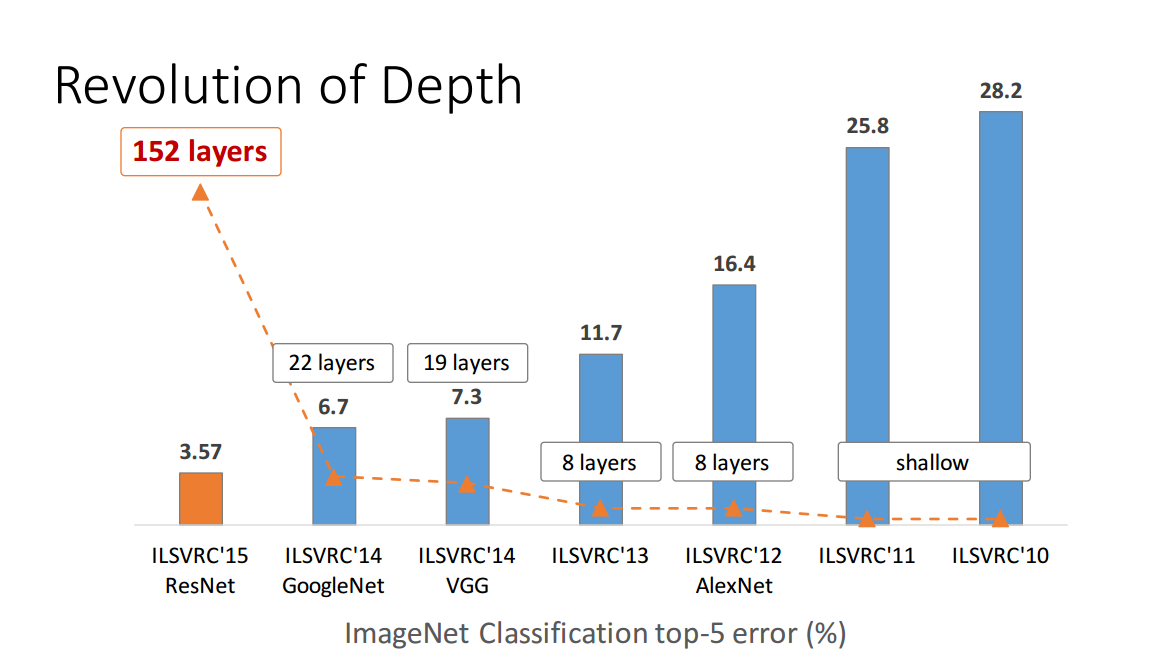
\includegraphics[scale=0.25]{cnn_power.png} \\
            	\scriptsize Source: Kaiming He, ICML 2016  \url{icml.cc/2016/tutorials/icml2016_tutorial_deep_residual_networks_kaiminghe.pdf}
            \end{figure} 
        \end{center}
    \end{frame}
    
    \begin{frame}[c]
    	\frametitle{Modern computer vision}
    	\begin{center}
    		\blue{CNNs} is the method of choice for many computer vision tasks. \\
    		\blue{We cannot ignore advances in the recent CNN development!}
    		
    		\begin{figure}
    			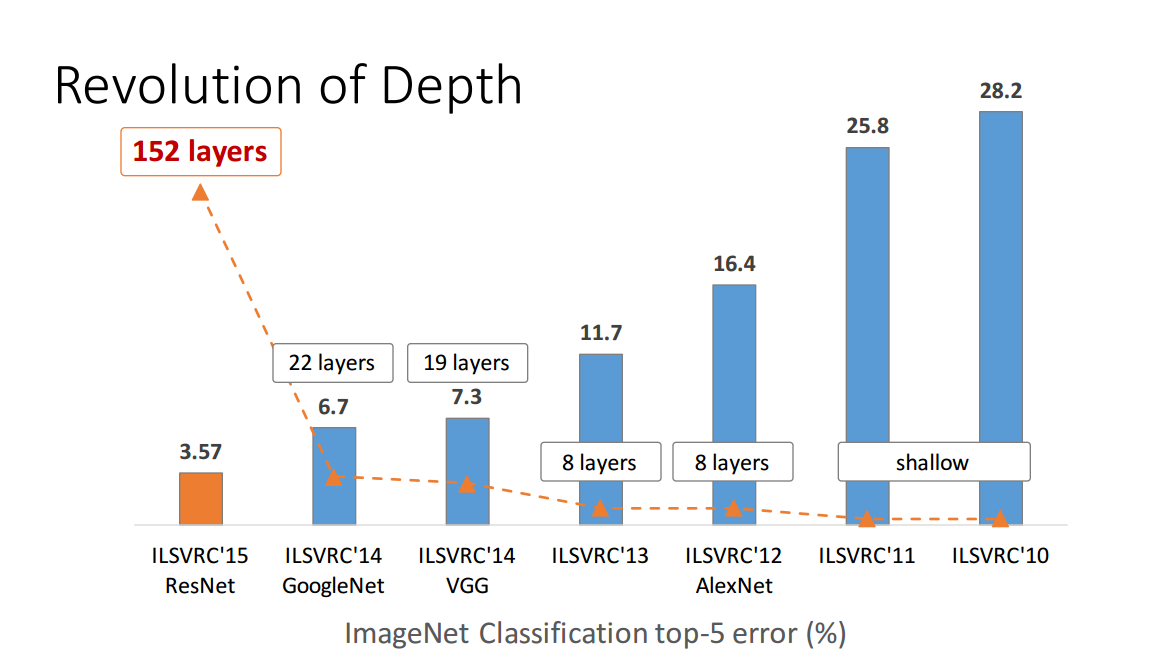
\includegraphics[scale=0.25]{cnn_power.png} \\
    			\scriptsize Source: Kaiming He, ICML 2016  \url{icml.cc/2016/tutorials/icml2016_tutorial_deep_residual_networks_kaiminghe.pdf}
    		\end{figure} 
    	\end{center}
    \end{frame}
    
    
    \begin{frame}[c]
       	\frametitle{Modern computer vision}
       	\begin{center}
       		Wait a moment, but what about \blue{PGMs}?
       	\end{center}
    \end{frame}
    
    \begin{frame}[c]
       	\frametitle{Modern computer vision}
       	\begin{center}
       		Wait a moment, but what about \blue{PGMs}? \\ \ \\
       		\red{Do we actually need them?}
       	\end{center}
    \end{frame}
    
    \begin{frame}[c]
       	\frametitle{Modern computer vision}
       	\begin{center}
       		Wait a moment, but what about \blue{PGMs}? \\ \ \\
       		\red{Do we actually need them?} \\ \ \\
       		Can \blue{CNNs} learn directly from data all needed relations between parts?
       	\end{center}
    \end{frame}
    
    
    \begin{frame}[c]
    	\frametitle{CNN part detector}
    	\begin{center}
    		Generally the results with a CNN part detector are quite \blue{good} \\
    		(we trained a CNN \textit{from scratch} on FLIC: 4000 images from movies)
    		\begin{figure}
    			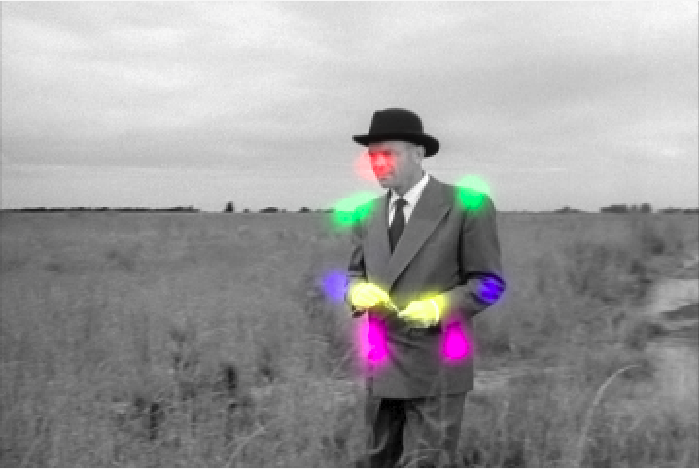
\includegraphics[scale=0.38]{cnn_pd_nice1.png} \\
    			\scriptsize Source: YF and MA
    		\end{figure} 
    	\end{center}
    \end{frame}

    \begin{frame}[c]
    	\frametitle{CNN part detector}
    	\begin{center}
    		Generally the results with a CNN part detector are quite \blue{good}
    		\begin{figure}
    			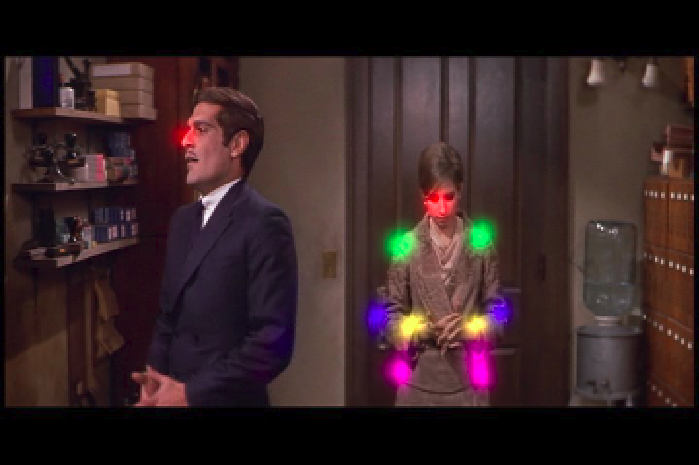
\includegraphics[scale=0.4]{cnn_pd_nice2.png} \\
    			\scriptsize Source: YF and MA
    		\end{figure} 
    	\end{center}
    \end{frame}
    
    
    \begin{frame}[c]
    	\frametitle{CNN part detector}
    	\begin{center}
    	But there are also quite \red{many false positives}! \\
    	(\textcolor{magenta}{pink} corresponds to a hip detection)
    		\begin{figure}
    			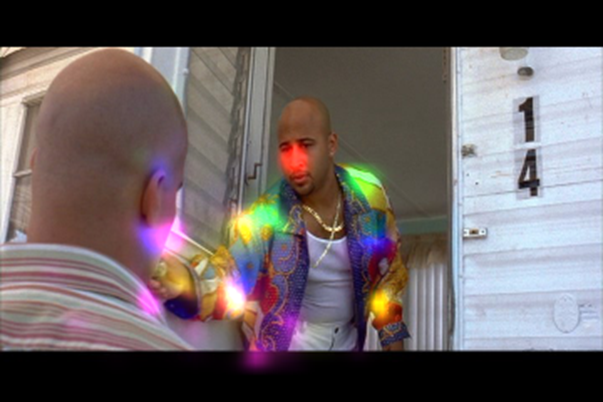
\includegraphics[scale=0.59]{false_positive.png} \\
    			\scriptsize Source: YF and MA.
    		\end{figure} 
    	\end{center}
    \end{frame}
    
    \begin{frame}[c]
       	\frametitle{CNN part detector}
       	\begin{center}
       		But there are also quite \red{many false positives}! \\
       		Some parts are hard, e.g. \textbf{right wrist detection} is problematic.
       		\begin{figure}
       			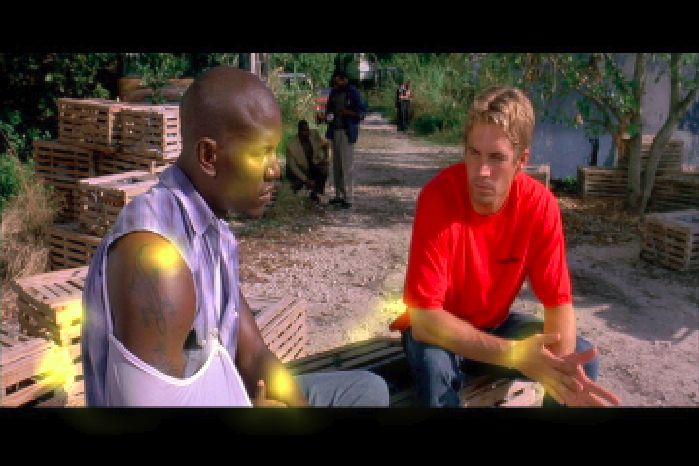
\includegraphics[scale=0.35]{cnn_pd_rwri_fail.png} \\
       			\scriptsize Source: YF and MA.
       		\end{figure} 
       	\end{center}
    \end{frame}


    \begin{frame}[c]
    	\frametitle{Solution?}
    	\begin{center}
    		What should we do with these \red{false positives}? \\ \ \\
    	\end{center}
    \end{frame}
    
    \begin{frame}[c]
    	\frametitle{Solution?}
    	\begin{center}
    		What should we do with these \red{false positives}? \\ \ \\
    		Use a PGM to enforce kinematic constraints! \\ \ \\
    	\end{center}
    \end{frame}
    
    \begin{frame}[c]
    	\frametitle{Solution?}
    	\begin{center}
    		What should we do with these \red{false positives}? \\ \ \\
    		Use a PGM to enforce kinematic constraints! \\ \ \\
    		So we can combine the best from 2 worlds: CNN and PGM. \\ \ \\
    	\end{center}
    \end{frame}
    
    \begin{frame}[c]
    	\frametitle{Solution?}
    	\begin{center}
    		What should we do with these \red{false positives}? \\ \ \\
    		Use a PGM to enforce kinematic constraints! \\ \ \\
    		So we can combine the best from 2 worlds: CNN and PGM. \\ \ \\
    		\blue{Moreover, we can train them jointly!}
    	\end{center}
    \end{frame}
    
    
    \begin{frame}[c]
    	\frametitle{CNN part detector}
   		\begin{figure}
   			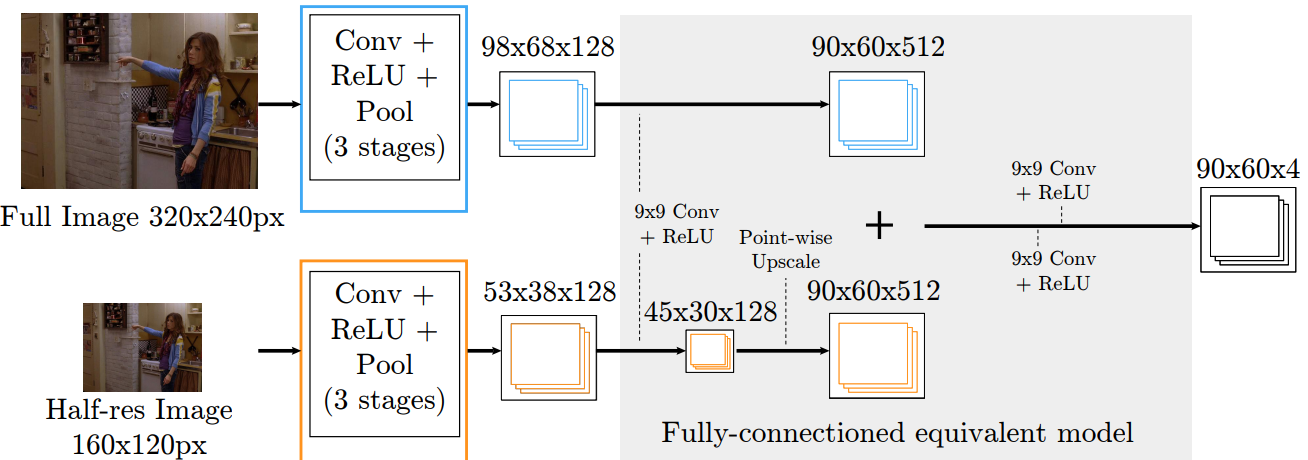
\includegraphics[scale=0.26]{cnn_architecture.png} \\
   			\scriptsize Source: "Joint Training of a CNN and a Graphical Model for Human Pose Estimation".
   		\end{figure} 
   		
   		How the \blue{CNN part detector} is implemented? $\rightarrow$ \blue{unary potentials} \\
   		\begin{itemize}
   			\item Coarse and fine resolution $\rightarrow$ 2 branches of the CNN
   			\item In the end: \textbf{softmax} and \textbf{MSE loss} to compare with the ground truth
   			\item We added \textbf{Batch Normalization}, which speeds up convergence \blue{x10 times}! $\rightarrow$ makes development of the project much faster
   			\item 6 convolutional layers is so 2014...
   		\end{itemize}
    \end{frame}


%we show how to actually detect parts! not just use black box probabilities (useful for fellow students)
%we learn spatial model instead of hardcoding it!
%approximation of MRF loopy belief propagation (not smth that we implemented in class)
%we use gradient-based optimization to find optimal parameters of the part-detector and of the spatial model 
%usually a PGM allows to correct false positives of a part detector
%here a PGM has a bias term (never seen before), which allows to correct false negatives by suggesting a part location based only on a pairwise compatibility => interesting idea!
%Note: we do single person pose estimation. For multi pose you should see [DeepCut: Joint Subset Partition and Labeling for Multi Person Pose Estimation] (https://arxiv.org/pdf/1511.06645.pdf), where they leverage graph clustering on top of a CNN part-detector.
%Question: how much overhead do we have with a fully-connected PGM? Of course, we have some overhead, but it doesn’t matter comparing with the time spent on the part detector.
%Exact reproducibility of their results is not possible!
%mistakes: size of images, size of feature maps after convolutions - how was it possible to make such mistakes?
%not much details: how to reproduce? 
%no description of the hyperparameters: learning rate, regularization coefficient, the variance of small gaussians in the heat map, random init
%even the optimization objective of the spatial model is unknown!
%not clear if they use softmax!
%the fact that they upscale 90x60 -> 360x240 for MSE (they mention it only as a comment for NIPS reviewers)
%they present 4 CNN models, describing a lot about them, however there is no clear answer why they don’t use 1x1 conv in the end
%Why not pre-trained model? we have to use the same architecture as in the paper! and there is no pre-trained model / code for it
%Emphasize: trained from scratch! on FLIC dataset, hps on our own

%feature maps: what patterns are learned
%weights of conv1: show as a sanity check
%big challenge: frontal vs back poses




	\begin{frame}[t]
        \frametitle{Higher-Level Spatial Model}
        \begin{center}
            \red{Problem}: Part Detector produces many false positives. \\ \ \\
			\blue{Solution}: use a Spatial Model to enforce the consistency.\\
        
         \begin{figure} % htbp stand for "here", "top", "bottom", "page"
            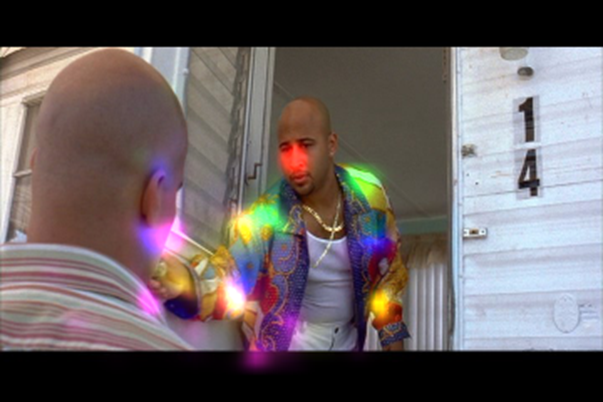
\includegraphics[scale=0.52]{false_positive.png} \\
            \scriptsize Source: YF and MA.
         \end{figure}
        \end{center}
    \end{frame}

	\begin{frame}[t]
        \frametitle{Spatial Model as a PGM}
        \begin{center}
			\blue{Traditional approach}: use the star model!\\
			What do we have for FLIC dataset?
            \begin{figure}[htbp] % htbp stand for "here", "top", "bottom", "page"
            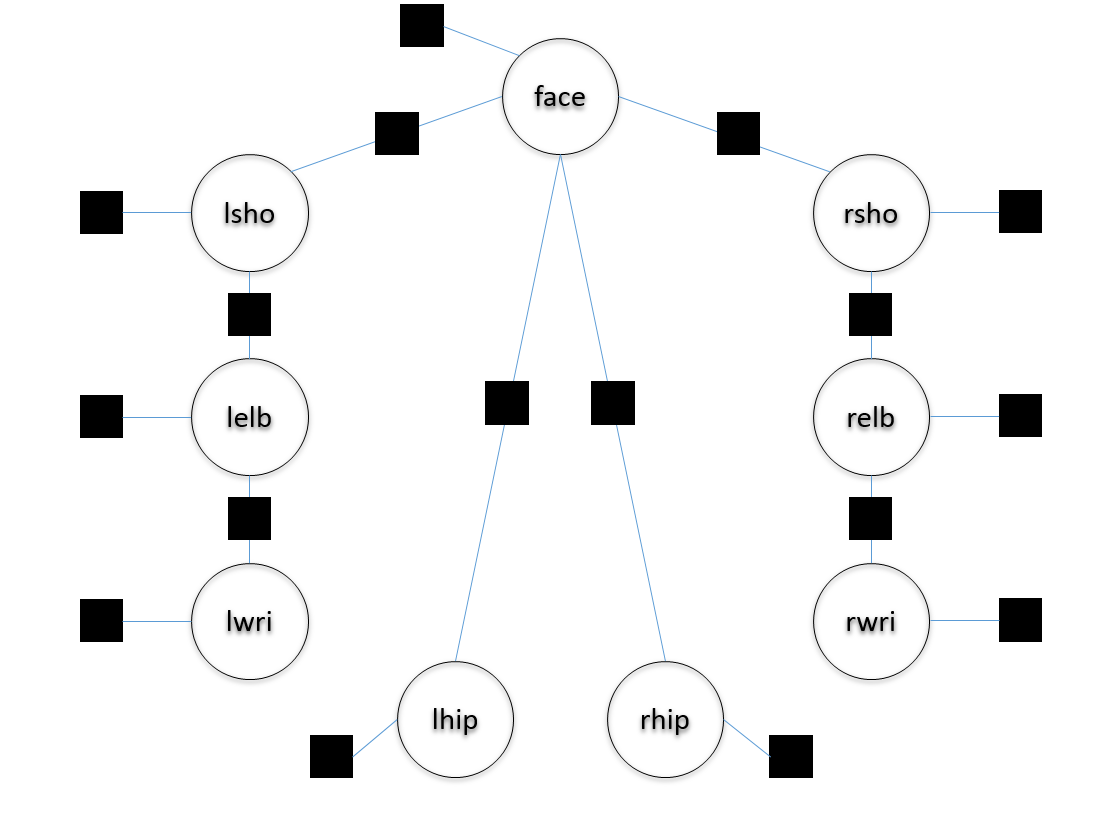
\includegraphics[scale=0.28]{star_model.png} \\
            \scriptsize Source: YF and MA.
            \end{figure}
        \end{center}
    \end{frame}
    
    
    \begin{frame}[t]
    	\frametitle{Spatial Model as a trainable PGM}
    	\begin{center}
    		\blue{But can we learn a PGM from data?} \\
    		$\rightarrow$ We should use \textbf{fully connected PGM} and train all potentials!
    		
    	\end{center}
    	
    	\begin{flushleft}
    		\textbf{Star PGM}:\\
    		\begin{itemize}
    			\item Computationally more efficient (during the train phase).\\
    			\item Less parameters to train.\\
    			\item Inference is exact.\\
    		\end{itemize}
    		\textbf{Fully Connected PGM}:\\
    		\begin{itemize}
    			\item More model capacity.\\
    			\item \blue{The model is learned from the data, no need of expert prior.}\\
    			\item Loopy structure has no guarantee of convergence.
    		\end{itemize}
    		
    		\blue{Fully connected PGM trained jointly with CNN} is the main novelty!
    	\end{flushleft}
    \end{frame}
    

	\begin{frame}[t]
        \frametitle{Inference in the fully connected PGM}
        \begin{center}
        	We do a single round of sum-product belief propagation to get marginals \\
        	\blue{Can be seen as approximation for Loopy Belief Propagation in MRF!}
            %$\hat{p}_{i} \propto p_{i} \prod_{u\in U}(p_{i|u}*p_u)$ \\
            %where U is a set of neighbouring nodes of body part i
            \begin{figure}[htbp] % htbp stand for "here", "top", "bottom", "page"
            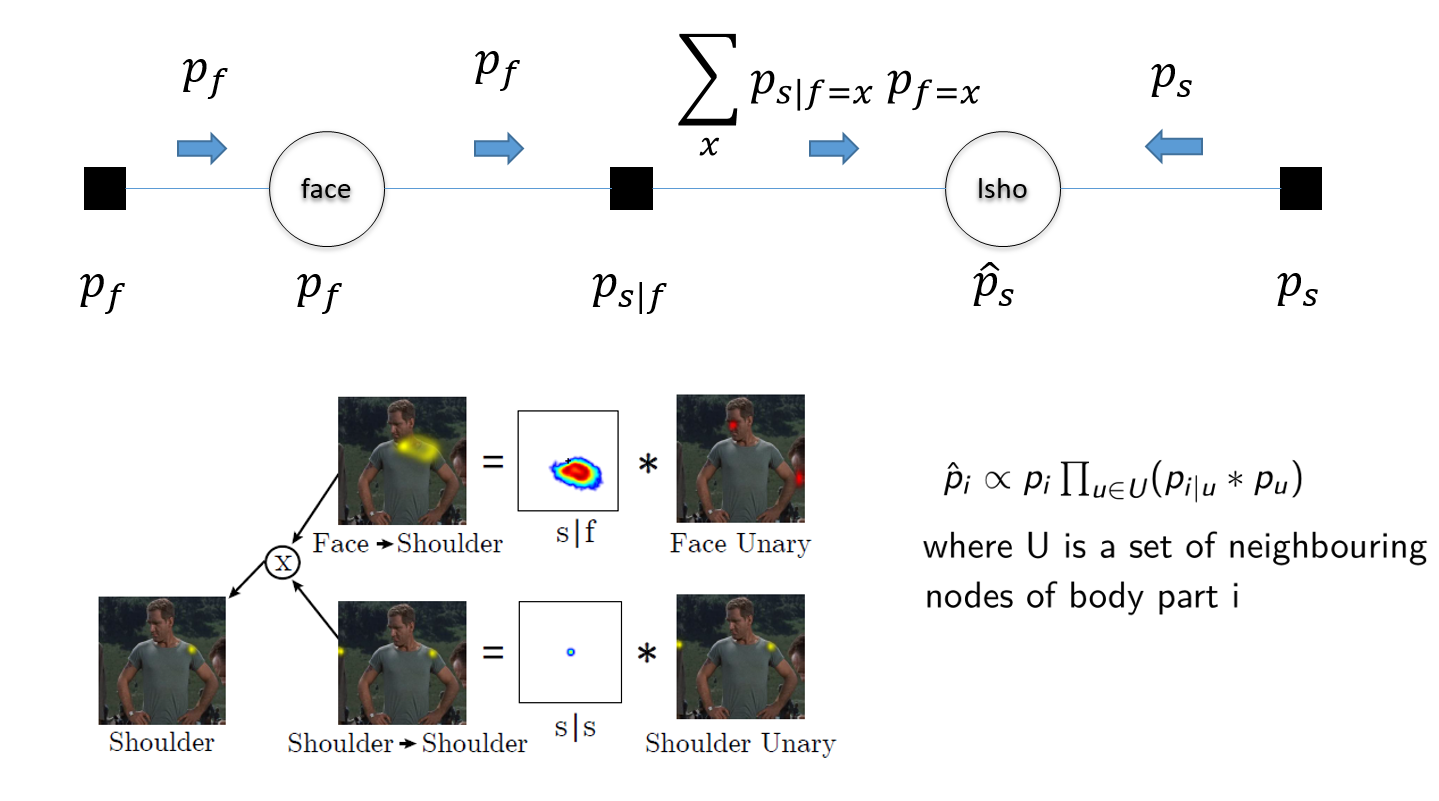
\includegraphics[scale=0.29]{inference.png} \\
            \scriptsize Source: YF, MA + "Joint Training of a CNN and a Graphical Model for HPE".
            \end{figure}
        \end{center}
    \end{frame}
    
    
    
    \begin{frame}[t]
    	\frametitle{Pairwise Potentials}
    	\begin{itemize}
    		\item Simple \red{$\mathcal{N}(\mu, \Sigma)$} doesn’t fit all the cases! (especially with diagonal $\Sigma$!) \\
    		\item We can learn this distribution in a non-parametric way (parametrized by 180x120 heat maps of pairwise compatibilities) by \blue{backprop}
    	\end{itemize}
    	\begin{center}
    		\begin{figure}[htbp] % htbp stand for "here", "top", "bottom", "page"
    			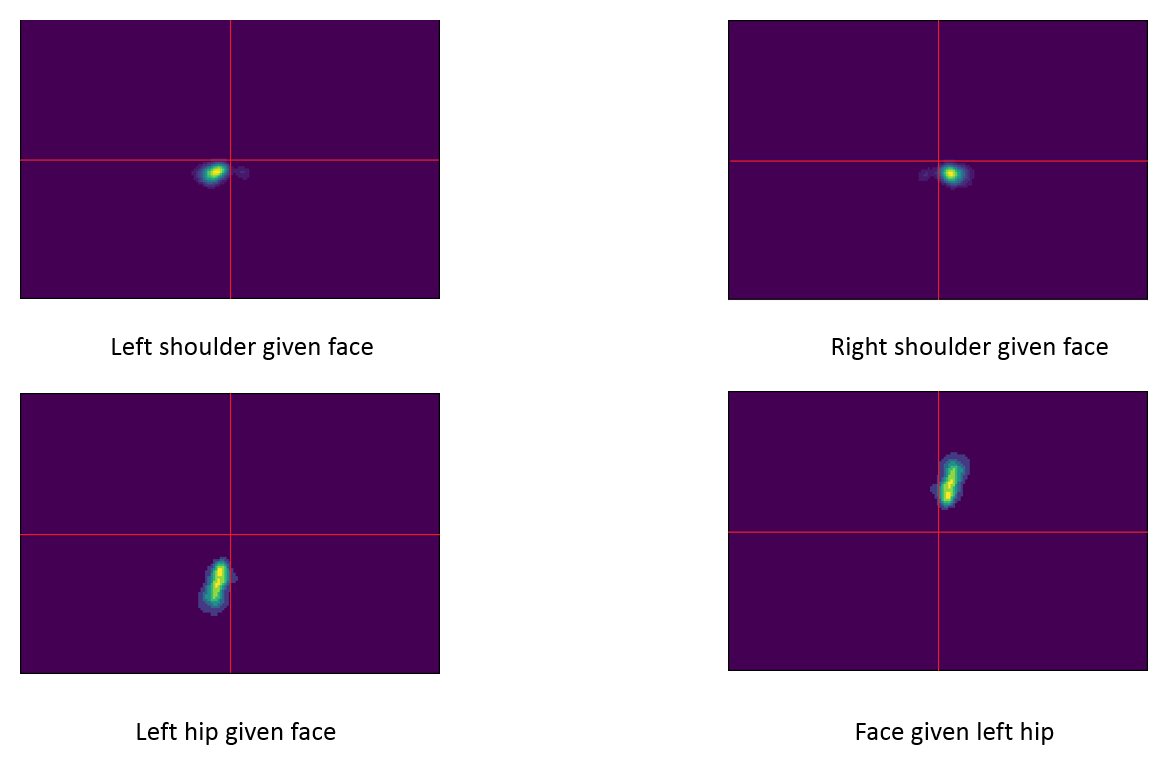
\includegraphics[scale=0.28]{pairwise_po.png} \\
    			\scriptsize We can use empirical histogram of joint displacements as \blue{good init}. Source: YF and MA.
    		\end{figure}
    	\end{center}
    \end{frame}


	\begin{frame}[t]
		\frametitle{Joint training}
		\begin{center}
			\blue{Joint training of the fully connected CNN and the PGM matters!}
			\begin{figure}
				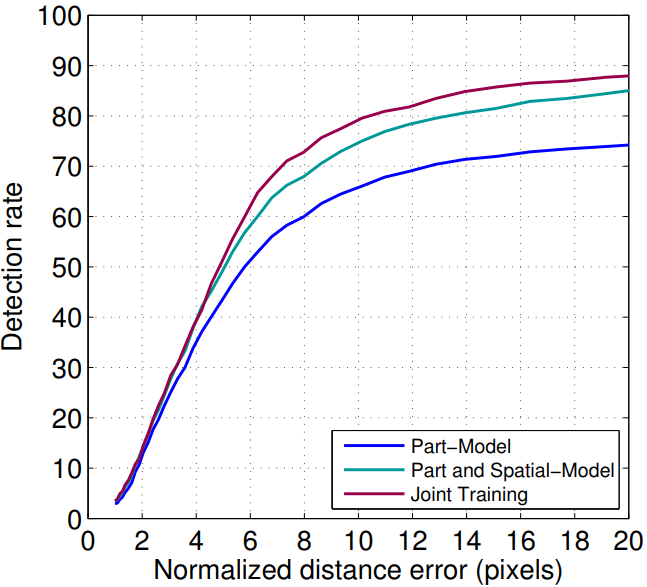
\includegraphics[scale=0.31]{joint_training_matters.png} \\
				\scriptsize Source: "Joint Training of a CNN and a Graphical Model for Human Pose Estimation".
			\end{figure}
		\end{center}
	\end{frame}
	
	
	\begin{frame}[t]
		\frametitle{State-of-the-art for 2014}
		\begin{center}
			\blue{The technique described above achieves the best results for 2014!}
			\begin{figure}
				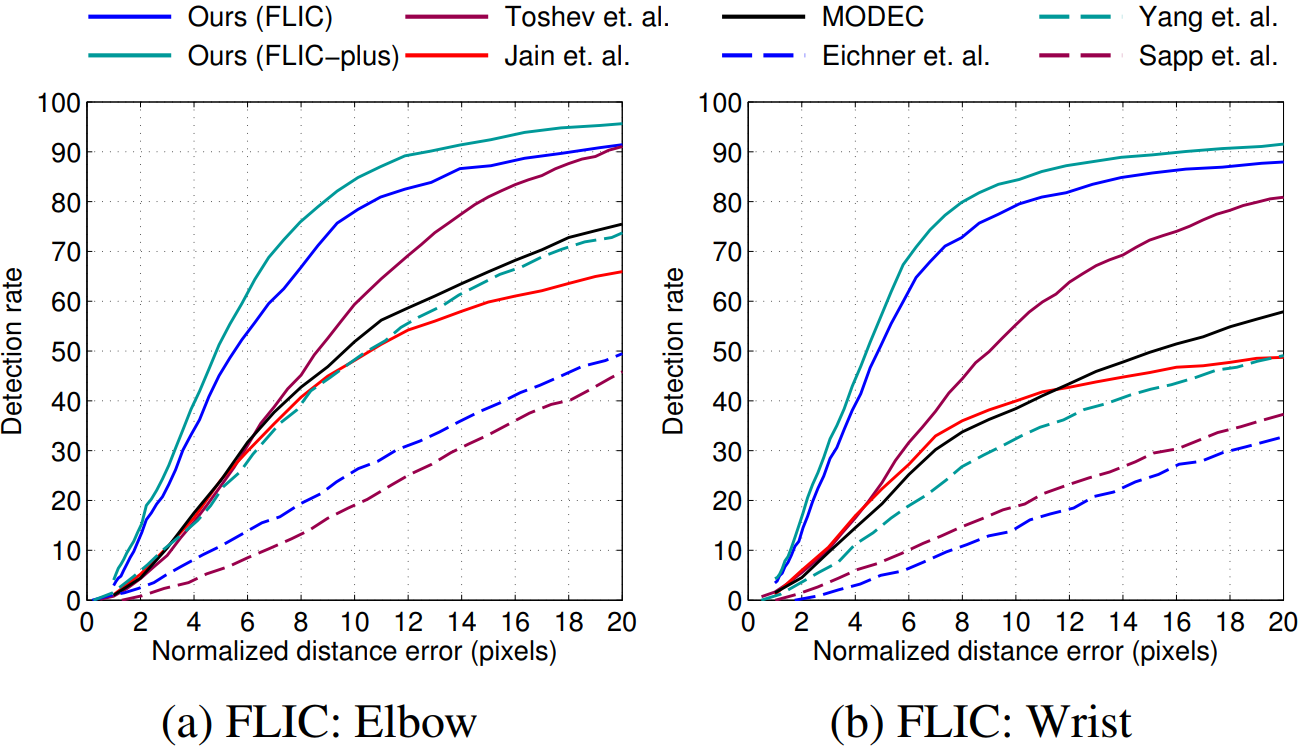
\includegraphics[scale=0.24]{sota.png} \\
				\scriptsize Source: "Joint Training of a CNN and a Graphical Model for Human Pose Estimation".
			\end{figure}
		\end{center}
	\end{frame}


    \begin{frame}[t]
        \frametitle{Final details}
        \begin{itemize}
            \item We open sourced all our code in our Github repository: \url{https://github.com/max-andr/cnn_mrf_hybrid_for_hpe}! \\
            \item Up to our knowledge, this is the first implementation of the presented paper \cite{cnn_pgm_for_hpe}.
            \item We extensively use TensorBoard! Now small demo.
        \end{itemize}
    \end{frame}


	\begin{frame}[plain,c]
		%\frametitle{A first slide}
		\begin{center}
			\Huge \blue{Thanks for your attention!} \\ \ \\
			Any questions? \\
		\end{center}
	\end{frame}
	
	
	\section*{References}
	\begin{thebibliography}{}
		\setbeamertemplate{bibliography item}[text]
		
		\bibitem{cnn_pgm_for_hpe}
		\href{https://arxiv.org/abs/1406.2984}
		{Joint Training of a Convolutional Network and a Graphical Model for Human Pose Estimation}

		\bibitem{cnn_pgm_for_hpe}
		\href{https://arxiv.org/abs/1312.7302}
		{Learning Human Pose Estimation Features with Convolutional Networks}
	\end{thebibliography} 
\end{document}